% ================== azurin.tex ===================
%Intramolecular electron transfer
\subsection{Intramolecular elctron transfer}
\begin{figure}
	\centering
	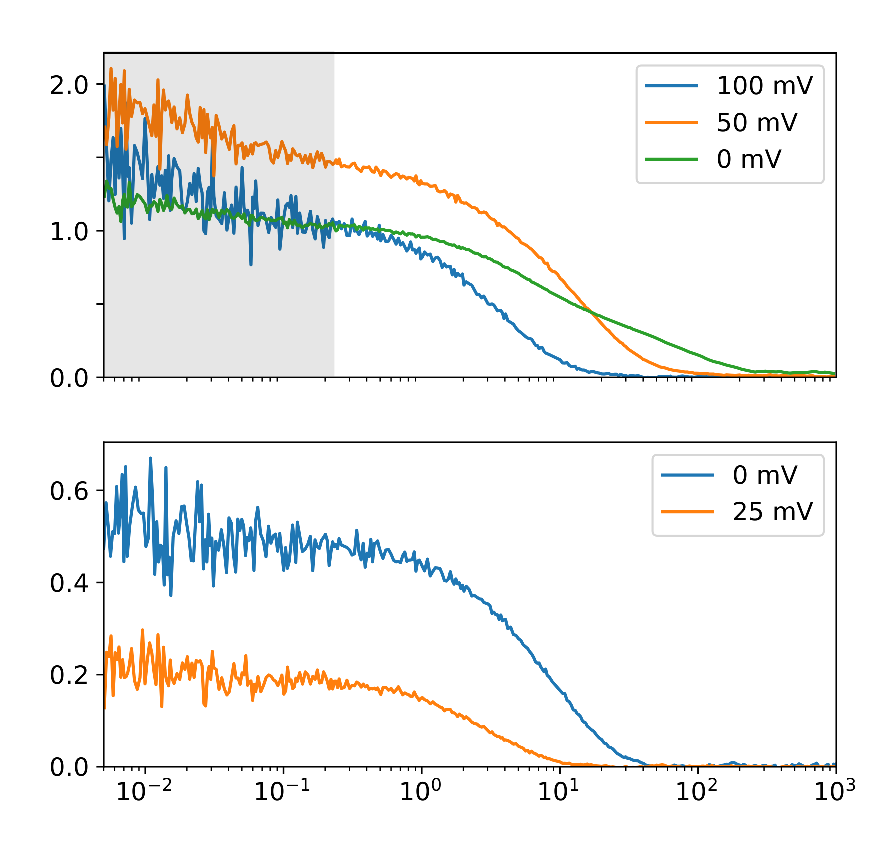
\includegraphics[width=0.6\textwidth]{fcs_components.eps}
	\caption{\textbf{Intra molecular electron transfer.} Shorter decay with time constant of around 30 us}
	\label{fig:fcs_components}
\end{figure}
%on-off 2D histogram
\begin{figure}
	\centering
	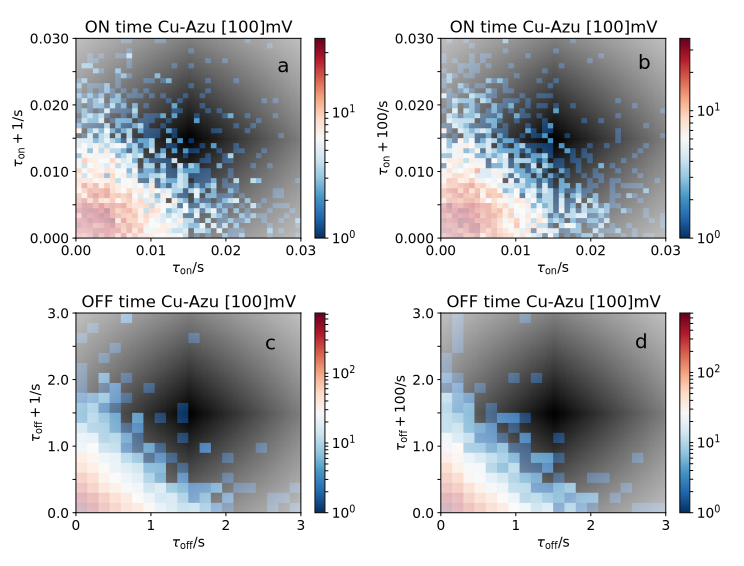
\includegraphics[width=\textwidth]{Figure_4_on_off_2D_100mV.png}
	\caption{\textbf{2D histogram: Cu-Azurin.} 2D correlation plot of (a) on-times vs the next on-times (b) on-times vs the on-time after 100 turnovers (c) off-times vs next off-times (d) off-times vs the off-time after 100 turnovers.}
	\label{fig:onoff2D}
\end{figure}
%Dynamic rates. protein showing diiferent rates with time
\subsection{Dynamics of ET rates}
\begin{figure}
	\centering
	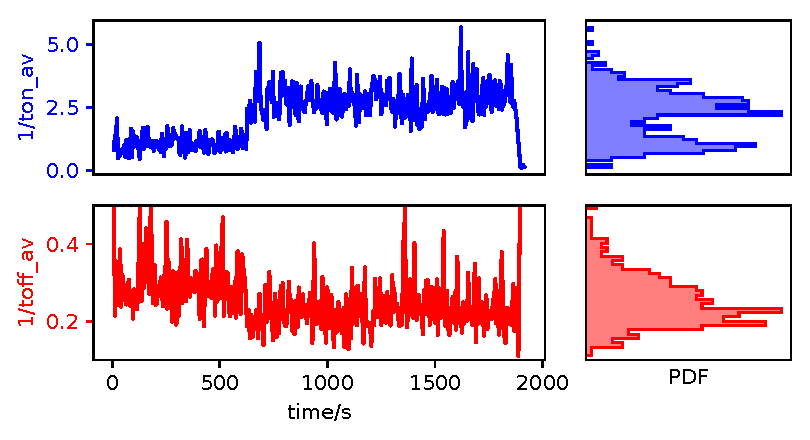
\includegraphics[width=\textwidth]{dynamic_rates.eps}
	\caption{\textbf{Dynamics in the turnovers of the protein.}}
	\label{fig:dynamic_rates}
\end{figure}

%===================Sup_info.tex======================
%2D on_off hist: ZnAzurin
\begin{figure}
  \centering
  \includegraphics[width=\textwidth,keepaspectratio]{Figure_SI/SI_on_off_2D_histogram_Zn.png}
	\makeatletter
	\renewcommand{\fnum@figure}{\figurename~S\thefigure}
	\makeatother
  \caption{\textbf{2D histogram: Zn-Azurin.} 2D correlation plot of (a) on-times vs the next on-times (b) on-times vs the on-time after 100 turnovers (c) off-times vs next off-times (d) off-times vs the off-time after 100 turnovers.}
  \label{SIfig:tracecomparision}
\end{figure}
%Cyclic voltametry: Electrochemical measurement
%commented out. will not appear in the compiled pdf
\iffalse
\begin{figure}
  \centering
  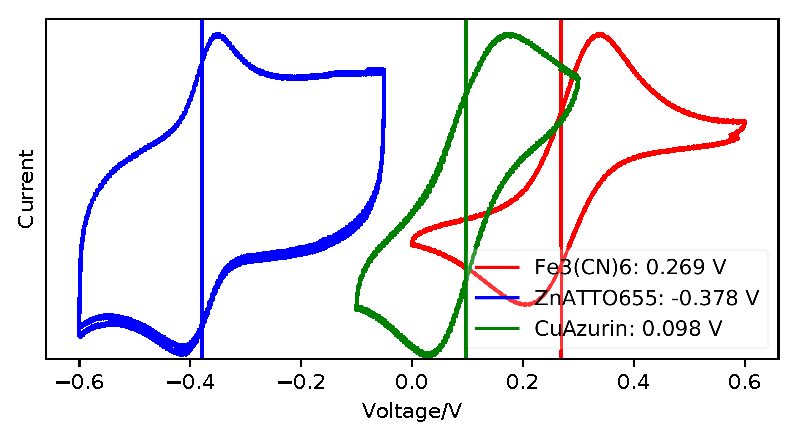
\includegraphics{cyclic_voltametry.eps}
  \makeatletter
  \renewcommand{\fnum@figure}{\figurename~S\thefigure}
  \makeatother
  \caption{Cyclic voltametry for Cu-Azurin (red), Pottasium Ferricyanide (green) and ATTO655 attached to ZnAzurin (blue). The mid point potential of Cuazurin is 98 mV.}
  \label{SIfig: cyclic_voltametry}
\end{figure}
\fi
%mid point potential of ZnAzurin
\begin{figure}
  \centering
  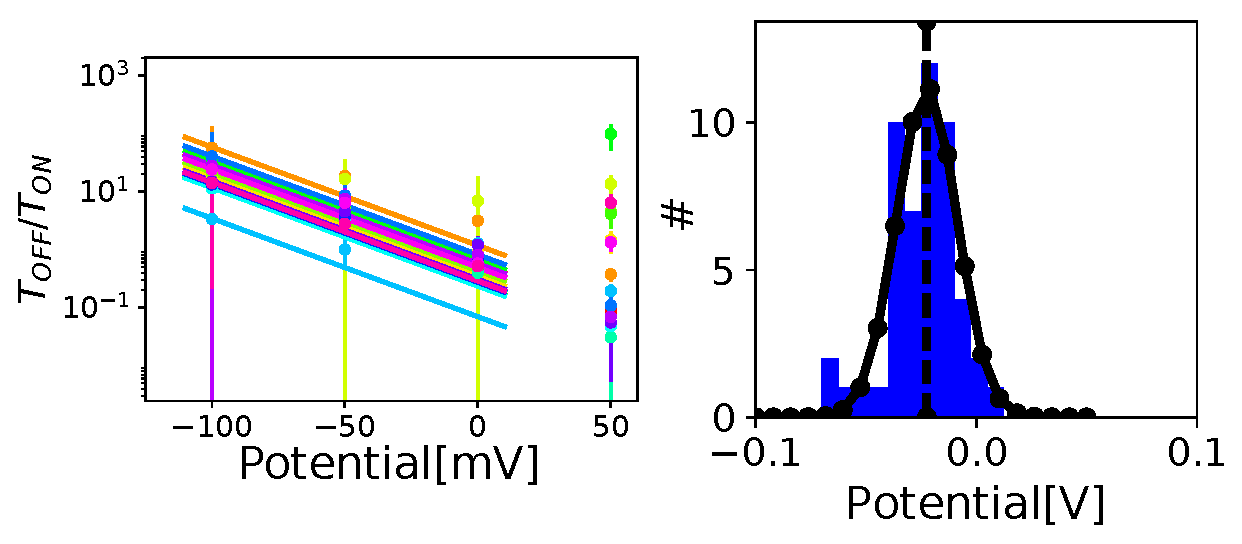
\includegraphics[width=\textwidth,keepaspectratio]{SI_potential_Zn.eps}
	\makeatletter
	\renewcommand{\fnum@figure}{\figurename~S\thefigure}
	\makeatother
  \caption{\textbf{Zn-AzurinATTO655 blinking.} Ratio between on and off time as a function of applied potential for the same single $ZnAzurin$ molecule. Different color represents different single-molecules. And the line connecting the data points is the Nernst fit for all the data points above 25 mV. The plot in the right is the histogram of midpoint potentials for $51$ molecules with a gaussian fit with center -23 mV with respect to calomel electrode.}
  \label{SIfig:2Dhist_Zn}
\end{figure}